\documentclass[conference]{IEEEtran}
\IEEEoverridecommandlockouts
\usepackage{cite}
\usepackage{amsmath,amssymb,amsfonts}
\usepackage{graphicx}
\usepackage{textcomp}
\usepackage{xcolor}
\usepackage{booktabs}
\usepackage{multirow}
\usepackage{array}
\usepackage{tabularx}
\usepackage{algorithm}
\usepackage{algorithmic}
\usepackage{tikz}
\usetikzlibrary{positioning,arrows.meta,fit,backgrounds,calc,shapes.geometric}
\usepackage[hidelinks]{hyperref}
\graphicspath{{figures/}}

% Float placement: let large figures sit at the top of a page without drifting.
\renewcommand{\topfraction}{0.92}
\renewcommand{\bottomfraction}{0.6}
\renewcommand{\textfraction}{0.07}
\renewcommand{\floatpagefraction}{0.75}
\renewcommand{\dbltopfraction}{0.92}
\renewcommand{\dblfloatpagefraction}{0.75}
\setcounter{topnumber}{3}
\setcounter{bottomnumber}{2}
\setcounter{totalnumber}{5}
\setcounter{dbltopnumber}{2}

\definecolor{ink}{HTML}{11222A}
\definecolor{teal}{HTML}{0A6970}
\definecolor{leak}{HTML}{B3412C}
\definecolor{slate}{HTML}{4F63A8}
\definecolor{mist}{HTML}{E6EEF0}
\definecolor{sand}{HTML}{F5E2DD}
\definecolor{fog}{HTML}{8A9AA0}

\newcommand{\auc}{\textsc{auc}}
\renewcommand{\algorithmicrequire}{\textbf{Input:}}
\renewcommand{\algorithmicensure}{\textbf{Output:}}

\begin{document}

\title{PimaLens: A Leakage-Free Benchmark of Dimensionality Reduction, Wrapper and Metaheuristic Feature Selection for Diabetes Screening on the Pima Indians Data}

\author{\IEEEauthorblockN{Ziad Elsayed Fouad\IEEEauthorrefmark{1}, Mohamed Adham Elhadidi\IEEEauthorrefmark{1}, Mohamed Hussien Kamal\IEEEauthorrefmark{1}}
\IEEEauthorblockA{\IEEEauthorrefmark{1}Faculty of Computer Science and Information Technology, Egypt-Japan University of Science and Technology, Alexandria, Egypt.\\
Email: \{ziad.320230025, mohamed.320230001, mohamed.320230008\}@ejust.edu.eg}}

\maketitle

\begin{abstract}
The Pima Indians diabetes data is one of the most reused benchmarks in clinical machine learning, and reported accuracies on it range from 72\% to above 95\%. We show how much of that spread can come from the evaluation itself. An earlier version of our own pipeline reported 87.8\% accuracy and an ROC-AUC of 0.942. An audit traced these numbers to two faults: the same 768 patients were stacked from two file versions, and one version filled missing insulin with the median of the patient's own diagnosis class, which predicts the label with an AUC of 1.000 on the 374 affected patients. We rebuilt the study on a checksum-verified copy of the raw data with a locked 20\% test set, one shared set of five stratified outer folds and nested inner cross-validation for every tuning and selection decision. On this protocol we compared all eight raw features against three linear reductions, eight nonlinear reductions, seven filter, wrapper and embedded selectors, and a genetic algorithm (GA) and binary particle swarm optimization (BPSO) that were scored against the exact optimum from an exhaustive search of all 255 feature subsets. No nonlinear reduction improved prediction for any of seven classifiers (best change $-0.026$ to $+0.001$ AUC). BPSO reached the exact optimum in 10 of 10 seeds with about a quarter of the exhaustive cost; the GA did so in 5 of 10. The selected model, logistic regression on four routine measurements, reached a cross-validated AUC of $0.846\pm0.015$ and accuracy of $79.2\%\pm1.9$, and an AUC of 0.811 (95\% CI 0.736 to 0.871) on the locked test set, where a pre-set screening threshold caught 48 of 54 diabetic patients. Re-estimated under the same protocol, the original 87.8\% pipeline scores 75.9\% accuracy.
\end{abstract}

\begin{IEEEkeywords}
data leakage, diabetes prediction, dimensionality reduction, feature selection, genetic algorithm, nested cross-validation, particle swarm optimization, t-SNE, UMAP
\end{IEEEkeywords}

%======================================================================
\section{Introduction}
%======================================================================

Type 2 diabetes is common and often diagnosed late, so a cheap screening rule built from routine measurements has practical value. The Pima Indians Diabetes Database, collected by the U.S. National Institute of Diabetes and Digestive and Kidney Diseases and released through the UCI repository in 1990, records eight such measurements for 768 women of Pima heritage aged 21 or older, 268 of whom tested positive for diabetes under World Health Organization criteria \cite{smith1988,uci_pima}. Its small size and clinical framing have made it a standard first dataset for new classifiers, feature selectors and optimizers.

The dataset is also harder than it looks. Five of its eight measurements use the value 0 to mean ``not recorded'': 48.7\% of patients have no insulin value and 29.6\% have no skin-fold value. Public ``cleaned'' copies fill these gaps in different ways, and some of those ways use the outcome. With only 768 patients, a single 80/20 split leaves a test set of about 150, on which one accuracy point is one or two patients. These properties make the benchmark easy to overfit at the level of the study design, through the choice of data version, split, threshold or model, even when each individual model is fitted correctly \cite{kapoor2023,cawley2010}.

This paper started as a course project whose first version reported 87.8\% accuracy and 0.942 AUC with a gradient-boosting model on five features chosen by a genetic algorithm. Those figures sit about ten points above the accuracy reported by careful single-classifier studies on the same data \cite{zou2018,chang2022}. We treated the gap as a question and audited the pipeline before comparing any methods. The audit, described in Section~\ref{sec:data}, found that the gap came from leakage. The rest of the paper rebuilds the study on a protocol designed so that every comparison is fair and every choice is made without the test set.

Within that protocol we ask three questions that the project brief raised and that the literature on this dataset usually answers under weaker evaluation:
\begin{enumerate}
\item Does nonlinear dimensionality reduction (Kernel PCA, SNE, t-SNE, UMAP, metric and non-metric MDS, Isomap, LLE) improve prediction over using all eight original measurements?
\item Do metaheuristic feature selectors such as a GA and binary PSO find the best feature subset, and at what cost, when the true optimum is known?
\item Which pipeline should be deployed for screening, and what does its honest performance look like?
\end{enumerate}

\begin{table*}[!t]
\centering
\caption{Related work on the Pima data. Each row was checked against the primary source or the dataset documentation. Scores are not directly comparable across rows because the patient set, missing-value handling and protocol differ.}
\label{tab:related}
\footnotesize
\begin{tabularx}{\textwidth}{@{}p{2.6cm}p{2.1cm}p{3.1cm}p{2.6cm}X@{}}
\toprule
Study & Patients & Method & Reported result & Protocol and limits on comparison \\
\midrule
Smith \textit{et al.} 1988 \cite{smith1988} & 768 & ADAP adaptive network & Sens.\ = spec.\ = 0.76 at cutoff 0.448 & One 576/192 split; no AUC. Verified from the UCI documentation and abstract; the body is a scanned PDF. \\
Zou \textit{et al.} 2018 \cite{zou2018} & 392 complete cases & RF, J48, NN with PCA or mRMR & RF + mRMR accuracy 0.7721 (0.7852 in their 10-fold table) & Five-fold CV. Dropping incomplete patients changes the population and removes the hardest cases. \\
Chang \textit{et al.} 2022 \cite{chang2022} & 768, median-imputed & Naive Bayes, RF, J48 & RF: acc.\ 79.57\%, AUC 0.862; NB (3 features): 79.13\% & One 70/30 split, no CV. Several RF metrics do not follow from the paper's own confusion matrices. \\
Hasan \textit{et al.} 2020 \cite{hasan2020} & 768 & AUC-weighted ensemble of 7 models & AUC 0.950, sens.\ 0.789, spec.\ 0.934 & K-fold CV with grid search. Fold count and nesting could not be confirmed from the accessible abstract; outlier rejection changes the patient set. \\
Original version of this project & 1,144 rows (two copies) & GA subset + tuned gradient boosting & Acc.\ 0.878, AUC 0.942 & Duplicate patients across the split, label-derived insulin, model and threshold chosen on the test set (Section~\ref{sec:data}). \\
\textbf{This work} & 768 verified & 181 pipelines on shared folds & CV AUC 0.846, acc.\ 0.792; test AUC 0.811 & Locked 20\% test, five outer folds, nested inner CV for every decision. \\
\bottomrule
\end{tabularx}
\end{table*}

The contributions are:
\begin{itemize}
\item A reproducible provenance and leakage audit of two widely circulated Pima file versions, showing that a class-conditional median fill produces a feature with AUC 1.000 on the affected rows and that stacking the two versions places 55.9\% of test rows next to their own copy in training.
\item A single evaluation protocol (locked test set, shared outer folds, nested inner CV, in-fold preprocessing) under which 181 pipelines are compared on identical patients.
\item A quantitative comparison of eleven dimensionality-reduction methods on the same patients by trustworthiness, runtime and class agreement, including a verified from-scratch symmetric SNE, and a predictive comparison of the seven methods that can embed new patients.
\item A GA versus BPSO comparison with equal objective, folds and evaluation budget, measured against the exact optimum from exhaustive search over all 255 subsets, under two different estimators and ten seeds each.
\item An honest final estimate with confusion matrices, a screening threshold set from out-of-fold predictions, bootstrap intervals, error analysis and a test-split diagnostic.
\end{itemize}

%======================================================================
\section{Related Work}
\label{sec:related}
%======================================================================

\subsection{Machine learning on the Pima data}
The dataset was introduced with the ADAP adaptive learning routine, trained on 576 patients and tested on 192, which reached equal sensitivity and specificity of 0.76 at a cutoff of 0.448 \cite{smith1988,uci_pima}. Later work spans most classifier families. Zou \textit{et al.} compared a decision tree, random forest (RF) and neural network with PCA and mRMR feature reduction; on Pima they removed patients with missing values, leaving 392, and reported a best five-fold accuracy of 0.7721 for RF on the mRMR subset of glucose, insulin and age \cite{zou2018}. Chang \textit{et al.} imputed invalid zeros with medians and evaluated naive Bayes, RF and J48 on one 70/30 split of 538 and 230 patients, reporting 79.57\% accuracy and an AUC of 0.862 for RF on all features and 79.13\% for naive Bayes on glucose, BMI and age \cite{chang2022}. Hasan \textit{et al.} combined outlier rejection, imputation, standardization and feature selection with an AUC-weighted ensemble of seven classifiers and reported an AUC of 0.950 with k-fold cross-validation and grid search \cite{hasan2020}. Table~\ref{tab:related} summarizes these studies and the limits on comparing them with ours.

\begin{figure*}[!t]
\centering
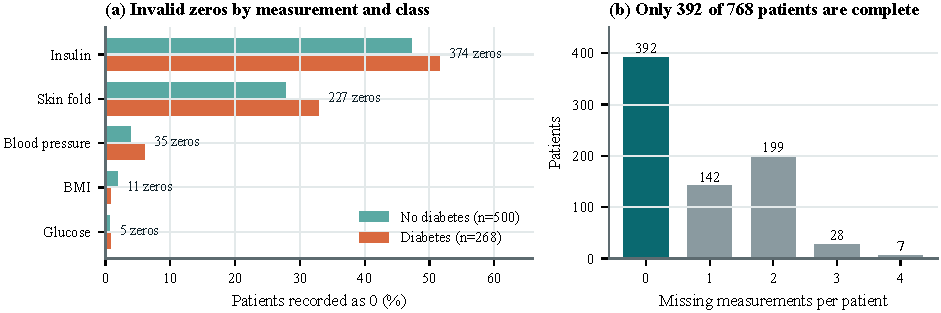
\includegraphics[width=\textwidth]{fig_missingness}
\caption{Missing values hidden as zeros. (a) Share of patients with an invalid zero by measurement and class. (b) Number of missing measurements per patient; fewer than half of all patients are complete cases, which is why studies that drop incomplete rows evaluate a different population.}
\label{fig:missing}
\end{figure*}

\subsection{Leakage and evaluation bias}
Leakage occurs when information that would not be available at prediction time enters training or model selection. Kapoor and Narayanan catalogued leakage across many applied fields and showed that it often inflates the apparent advantage of complex models \cite{kapoor2023}. Two forms matter here. Preprocessing that uses the label, such as class-conditional imputation, creates features that encode the outcome. Selection on the evaluation data, such as choosing the model or threshold on the test set or selecting features on all the data before cross-validation, biases the estimate even when the data is clean \cite{ambroise2002,varma2006,cawley2010}. Nested cross-validation, in which every data-driven choice is repeated inside each training fold, removes the second form \cite{varma2006}.

\subsection{Dimensionality reduction}
Linear projections (PCA, truncated SVD and LDA) remain the default for tabular data. Nonlinear methods either preserve global geometry (Kernel PCA \cite{scholkopf1998}, metric and non-metric MDS \cite{kruskal1964}, Isomap \cite{tenenbaum2000}) or local neighbourhoods (LLE \cite{roweis2000}, SNE \cite{hinton2002}, t-SNE \cite{vandermaaten2008}, UMAP \cite{mcinnes2018}). Neighbourhood methods are mainly visualization tools; t-SNE and classical MDS have no mapping for new points, so their coordinates cannot be used to score unseen patients without a separate out-of-sample method. Trustworthiness \cite{venna2001} measures how many of a point's neighbours in the embedding were also neighbours in the input space, and gives a quantitative basis for comparing embeddings.

\subsection{Metaheuristic feature selection}
Wrapper selection searches subsets of features using the cross-validated score of a model as the objective. Population-based searches, especially GAs \cite{holland1975} and binary PSO \cite{kennedy1997}, are widely used for this and are surveyed by Xue \textit{et al.} \cite{xue2016}. Most studies compare metaheuristics with each other or with sequential search. With eight features, the full space has only $2^8-1=255$ subsets, so exhaustive search is affordable and gives the exact optimum of the objective. That allows the quality of each metaheuristic to be measured as a gap to a known optimum, which is rarely possible on larger problems.

%======================================================================
\section{Data and Provenance Audit}
\label{sec:data}
%======================================================================

\begin{figure*}[!t]
\centering
\resizebox{\textwidth}{!}{%
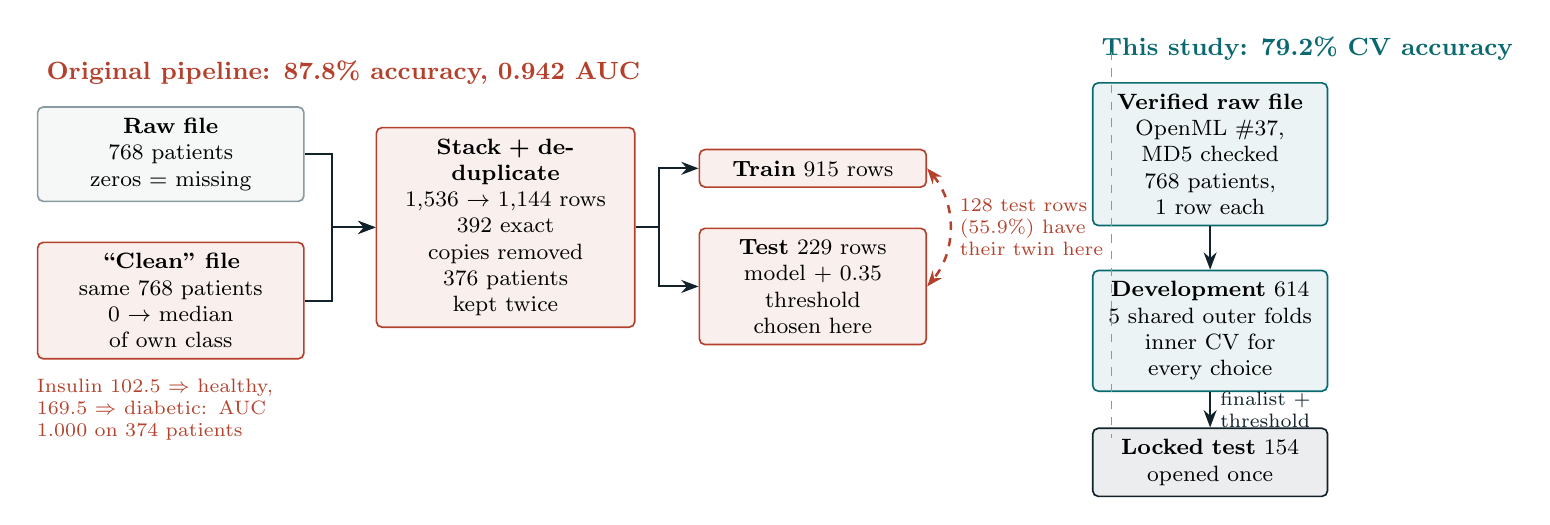
\begin{tikzpicture}[
  font=\footnotesize,
  box/.style={draw=#1, fill=#1!8, rounded corners=2pt, align=center, inner sep=4pt, line width=0.6pt},
  box/.default=ink,
  arr/.style={-{Stealth[length=2.2mm]}, line width=0.7pt, draw=ink},
  note/.style={align=left, font=\scriptsize, text=ink}]
% ---------- left: original pipeline
\node[box=fog, text width=3.1cm] (raw) {\textbf{Raw file}\\768 patients\\zeros = missing};
\node[box=leak, text width=3.1cm, below=0.5cm of raw] (clean) {\textbf{``Clean'' file}\\same 768 patients\\0 $\rightarrow$ median of own class};
\coordinate (mid) at ($(raw.east)!0.5!(clean.east)$);
\node[box=leak, text width=3.0cm, right=0.9cm of mid, anchor=west] (merge) {\textbf{Stack + de-duplicate}\\1,536 $\rightarrow$ 1,144 rows\\392 exact copies removed\\376 patients kept twice};
\node[box=leak, text width=2.6cm, right=0.8cm of merge, yshift=0.75cm] (train) {\textbf{Train} 915 rows};
\node[box=leak, text width=2.6cm, right=0.8cm of merge, yshift=-0.75cm] (test) {\textbf{Test} 229 rows\\model + 0.35 threshold\\chosen here};
\draw[arr] (raw.east) -- ++(0.35,0) |- (merge.west);
\draw[arr] (clean.east) -- ++(0.35,0) |- (merge.west);
\draw[arr] (merge.east) -- ++(0.3,0) |- (train.west);
\draw[arr] (merge.east) -- ++(0.3,0) |- (test.west);
\draw[leak, line width=0.9pt, dashed, {Stealth[length=2mm]}-{Stealth[length=2mm]}] (train.east) to[bend left=40] node[right, note, text=leak]{128 test rows\\(55.9\%) have\\their twin here} (test.east);
\node[note, text=leak, below=0.12cm of clean, text width=3.4cm] {Insulin 102.5 $\Rightarrow$ healthy,\\169.5 $\Rightarrow$ diabetic: AUC 1.000 on 374 patients};
\node[font=\small\bfseries, text=leak, above=0.15cm of raw.north west, anchor=south west] {Original pipeline: 87.8\% accuracy, 0.942 AUC};
% ---------- right: corrected pipeline
\begin{scope}[xshift=13.2cm]
\node[box=teal, text width=2.7cm] (vraw) {\textbf{Verified raw file}\\OpenML \#37, MD5 checked\\768 patients, 1 row each};
\node[box=teal, text width=2.7cm, below=0.55cm of vraw] (vdev) {\textbf{Development} 614\\5 shared outer folds\\inner CV for every choice};
\node[box=ink, text width=2.7cm, below=0.45cm of vdev] (vtest) {\textbf{Locked test} 154\\opened once};
\draw[arr] (vraw) -- (vdev); \draw[arr] (vdev) -- node[right, note]{finalist +\\threshold} (vtest);
\node[font=\small\bfseries, text=teal, above=0.15cm of vraw.north west, anchor=south west] {This study: 79.2\% CV accuracy};
\end{scope}
\draw[fog, line width=0.5pt, dashed] (11.95,1.3) -- (11.95,-3.6);
\end{tikzpicture}}
\caption{How the original pipeline leaked (left) and the corrected design (right). Two copies of the same patients were stacked; the cleaned copy encoded the diagnosis in its filled values; and most test rows had a copy of their own patient in training. Re-estimated under the corrected design, the same modelling choices give 75.9\% accuracy and 0.829 AUC (Section~\ref{sec:results}).}
\label{fig:leakdiagram}
\vspace{2mm}
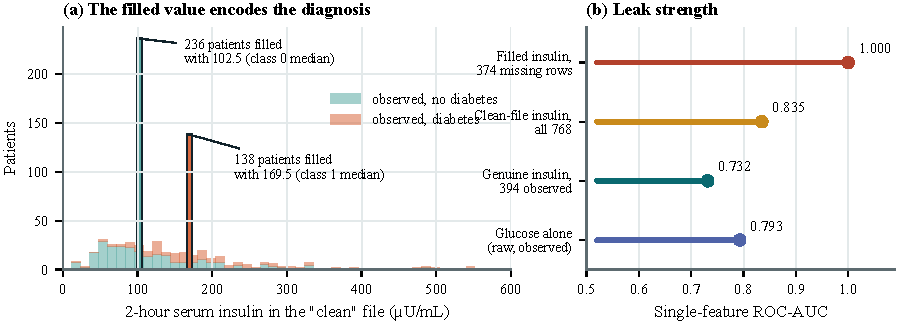
\includegraphics[width=\textwidth]{fig_leak}
\caption{Evidence for the label leak. (a) Insulin in the cleaned file: the 374 missing values become two spikes at the class medians. (b) Single-feature ROC-AUC. The filled insulin values alone identify the diagnosis perfectly on the rows where insulin was missing, far above what genuine insulin or glucose achieve.}
\label{fig:leak}
\end{figure*}

\subsection{Dataset}
Table~\ref{tab:data} lists the eight measurements. The outcome is a positive diabetes test (268 of 768, 34.9\%). Pregnancies, the pedigree function and age are always recorded. Zeros in the other five columns are physiologically impossible and encode missing values (Fig.~\ref{fig:missing}). Only 392 patients (51.0\%) have all five; 199 lack two. Missingness is slightly more common among diabetic patients for insulin, skin fold and blood pressure.

\begin{table}[!tb]
\centering
\caption{Measurements in the Pima data and the share recorded as an invalid zero (all 768 patients).}
\label{tab:data}
\footnotesize
\begin{tabular}{@{}llrr@{}}
\toprule
Feature & Unit & Invalid 0 & Univariate AUC$^\dagger$ \\
\midrule
Pregnancies & count & n/a (111 real 0) & 0.610 \\
Glucose (2-h OGTT) & mg/dL & 5 (0.7\%) & 0.799 \\
Diastolic blood pressure & mm Hg & 35 (4.6\%) & 0.618 \\
Triceps skin fold & mm & 227 (29.6\%) & 0.665 \\
2-h serum insulin & $\mu$U/mL & 374 (48.7\%) & 0.772 \\
BMI & kg/m$^2$ & 11 (1.4\%) & 0.694 \\
Diabetes pedigree (DPF) & index & n/a & 0.604 \\
Age & years & n/a & 0.682 \\
\bottomrule
\multicolumn{4}{@{}l}{\scriptsize $^\dagger$ On the 614 development patients after in-fold imputation; descriptive only.}
\end{tabular}
\end{table}

\subsection{Provenance verification}
The original project files were not available when this study started, so the raw data was re-obtained from OpenML (dataset 37, version 1). Its MD5 checksum matched the value OpenML publishes for the file, and every row and label matched an independent mirror of the UCI file \texttt{pima-indians-diabetes.data}. The UCI documentation confirms 768 instances and a 500/268 class split \cite{uci_pima}. The analysis notebook repeats these checks on every run and stops if any fails.

\subsection{Anatomy of the original leak}
The original pipeline loaded two files, a raw copy and a ``cleaned'' copy, stacked them into 1,536 rows and removed exact duplicates to get 1,144. Fig.~\ref{fig:leakdiagram} traces what happened. Three checks established it:

\textit{Same patients.} In both files, the columns that are never zero (pregnancies, pedigree, age and the outcome) agree for all 768 rows in the same order, and every non-zero measurement agrees. The 392 complete-case patients are byte-identical in both files, which is exactly the number of rows the de-duplication removed. The remaining 376 patients appear twice: once with gaps and once with filled values.

\textit{Label-derived fill.} In the cleaned copy every invalid zero is replaced by a single value per class, equal to the median of the observed values among patients with the same diagnosis (for insulin, 102.5 for negatives and 169.5 for positives; Fig.~\ref{fig:leak}a). Among the 374 patients whose real insulin is missing, the filled value alone separates the classes perfectly (AUC 1.000; Fig.~\ref{fig:leak}b). Genuine insulin, where it was measured, reaches 0.732. Rebuilding the cleaned file with this rule reproduced the original notebook's merged table exactly: 1,144 rows, and the count and mean of every column within $5\times10^{-7}$. The original file itself could not be compared byte for byte.

\textit{Twins across the split.} Repeating the original stratified split on the merged table shows that 128 of its 229 test rows (55.9\%) had their own patient in the training set, usually in the leaked version. The model and the screening threshold of 0.35 had also been chosen from test-set results.

\textit{Decision.} All analyses below use only the verified raw file, with one row per patient. The cleaned file is never used for training or evaluation.

%======================================================================
\section{Methodology}
\label{sec:method}
%======================================================================

\subsection{Evaluation protocol}
Fig.~\ref{fig:protocol} shows the protocol. A stratified 20\% test set of 154 patients (54 positive) is drawn with a fixed seed and stored in an object that can be opened only once. The remaining 614 development patients are split into five stratified outer folds that every comparable experiment shares, so two pipelines are always compared on the same patients. Any decision that uses data, such as a hyperparameter, a feature subset, a regularization strength or a number of retained features, is made by inner five-fold cross-validation within the outer training fold. The outer validation fold is used only for scoring.

The following rules were fixed before any model was scored. The primary ranking metric is the mean outer five-fold ROC-AUC, because it does not depend on a threshold. Mean five-fold accuracy is reported beside it, as the course rubric requires. The finalist is the pipeline with the highest mean CV AUC; ties within 0.001 go to the pipeline needing fewer raw measurements, then to the simpler model. The screening threshold is the highest threshold whose out-of-fold recall on the development set is at least 0.85. A feature must earn at least 0.002 AUC to be kept; this tolerance appears in the sequential selectors, the filter's $k$ rule and the metaheuristic penalty.

\begin{figure}[!tb]
\centering
\resizebox{\columnwidth}{!}{%
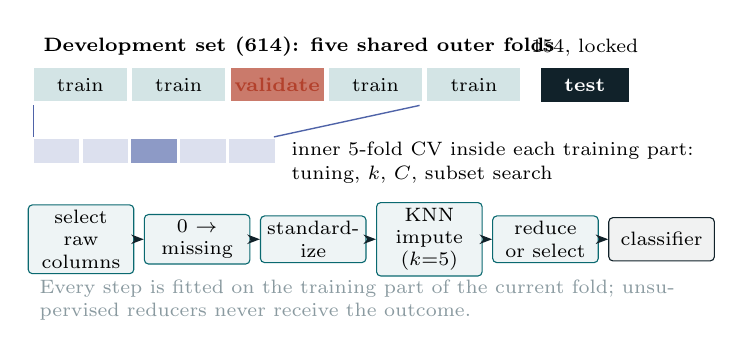
\begin{tikzpicture}[font=\scriptsize,
  st/.style={draw=teal, fill=teal!7, rounded corners=1.5pt, minimum height=0.55cm, text width=1.2cm, align=center, inner sep=2pt},
  arr/.style={-{Stealth[length=1.6mm]}, line width=0.6pt, draw=ink}]
% data bar
\foreach \i in {0,...,4} {
  \fill[teal!18] (\i*1.25,0) rectangle ++(1.18,0.42);
}
\fill[leak!70] (2*1.25,0) rectangle ++(1.18,0.42);
\node[font=\scriptsize\bfseries, anchor=south west] at (0,0.45) {Development set (614): five shared outer folds};
\node[font=\scriptsize, text=leak] at (2*1.25+0.59,0.21) {\textbf{validate}};
\foreach \i/\l in {0/train,1/train,3/train,4/train} { \node[font=\scriptsize] at (\i*1.25+0.59,0.21) {\l}; }
\draw[fill=ink, draw=ink] (6.45,0) rectangle ++(1.1,0.42); \node[text=white] at (7.0,0.21) {\textbf{test}};
\node[font=\scriptsize, anchor=south] at (7.0,0.45) {154, locked};
% inner CV
\foreach \i in {0,...,4} { \fill[slate!20] (\i*0.62,-0.78) rectangle ++(0.58,0.3); }
\fill[slate!65] (1.24,-0.78) rectangle ++(0.58,0.3);
\node[anchor=west] at (3.15,-0.63) {inner 5-fold CV inside each training part:};
\node[anchor=west] at (3.15,-0.93) {tuning, $k$, $C$, subset search};
\draw[slate, line width=0.5pt] (0,-0.05) -- (0,-0.45); \draw[slate, line width=0.5pt] (4.9,-0.05) -- (3.05,-0.45);
% pipeline
\node[st] (a) at (0.6,-1.75) {select raw columns};
\node[st, right=0.12cm of a] (b) {0 $\rightarrow$ missing};
\node[st, right=0.12cm of b] (c) {standard\-ize};
\node[st, right=0.12cm of c] (d) {KNN impute ($k{=}5$)};
\node[st, right=0.12cm of d] (e) {reduce or select};
\node[st, right=0.12cm of e, draw=ink, fill=ink!6] (f) {classifier};
\foreach \x/\y in {a/b,b/c,c/d,d/e,e/f} { \draw[arr] (\x) -- (\y); }
\node[anchor=north west, align=left, text=fog, text width=8.4cm] at (-0.05,-2.15) {Every step is fitted on the training part of the current fold; unsupervised reducers never receive the outcome.};
\end{tikzpicture}}
\caption{Evaluation protocol. All pipelines share the same outer folds; every data-driven choice is repeated on inner folds; the test set is opened once for the locked finalist. The in-fold pipeline drops columns before imputation, so a dropped measurement cannot influence predictions.}
\label{fig:protocol}
\end{figure}

\subsection{Preprocessing}
Each pipeline begins with four fitted steps: keep the requested raw columns, recode invalid zeros as missing, standardize, then impute with $k$-nearest-neighbour imputation \cite{troyanskaya2001} ($k=5$) in the standardized space. All four are fitted on the training part of the current fold. Selecting columns before imputation matters for claims about fewer measurements: if a column were dropped after imputation, its values would still have shaped the imputed values of the columns that remain.

\subsection{Linear dimensionality reduction}
PCA projects onto the leading eigenvectors of the covariance matrix. Truncated SVD factorizes the data without centring; on standardized data the two nearly coincide. LDA finds the projection that maximizes between-class to within-class scatter; for two classes it has exactly one axis. PCA and SVD are evaluated at two and four components, LDA at one.

\subsection{Nonlinear dimensionality reduction}
Kernel PCA uses an RBF kernel with $\gamma=0.1$ \cite{scholkopf1998}. Isomap \cite{tenenbaum2000} and LLE \cite{roweis2000} use 15 neighbours; UMAP \cite{mcinnes2018} uses 15 neighbours and a minimum distance of 0.1; t-SNE \cite{vandermaaten2008} uses perplexity 30 and PCA initialization. Metric and non-metric MDS \cite{kruskal1964} start from classical MDS. Every unsupervised reducer is wrapped so that the outcome is never passed to its \texttt{fit} method; without this wrapper a scikit-learn pipeline passes $y$ to UMAP, which then silently runs its supervised variant.

\textit{Symmetric SNE.} We implemented SNE from scratch. High-dimensional affinities use a Gaussian kernel whose bandwidth $\sigma_i$ is set by binary search so that the perplexity of $p_{j|i}$ equals 30, and are symmetrized:
\begin{equation}
p_{j|i}=\frac{\exp(-\lVert x_i-x_j\rVert^2/2\sigma_i^2)}{\sum_{k\neq i}\exp(-\lVert x_i-x_k\rVert^2/2\sigma_i^2)},\qquad p_{ij}=\frac{p_{j|i}+p_{i|j}}{2n}.
\end{equation}
Low-dimensional affinities use a joint Gaussian, and the embedding minimizes the Kullback--Leibler divergence:
\begin{equation}
q_{ij}=\frac{\exp(-\lVert y_i-y_j\rVert^2)}{\sum_{k\neq l}\exp(-\lVert y_k-y_l\rVert^2)},\qquad C=\sum_{i\neq j}p_{ij}\log\frac{p_{ij}}{q_{ij}},
\end{equation}
with gradient
\begin{equation}
\frac{\partial C}{\partial y_i}=4\sum_{j}(p_{ij}-q_{ij})(y_i-y_j).
\label{eq:snegrad}
\end{equation}
This is the symmetric variant of SNE \cite{vandermaaten2008}, which differs from the original asymmetric SNE \cite{hinton2002} in using a joint $q_{ij}$, and from t-SNE only in its Gaussian (rather than Student-$t$) low-dimensional kernel. Optimization uses gradient descent with learning rate 200, momentum 0.5 for 250 iterations then 0.8, gradient-norm clipping at 100 and 1,000 iterations. Three checks confirm the implementation: achieved perplexities equal the target to four decimals; the analytic gradient \eqref{eq:snegrad} matches a central finite-difference gradient of $C$ with relative error $2\times10^{-10}$; and $C$ falls from 2.86 to 1.33.

\textit{Embedding quality.} All eleven methods embed the same 614 standardized, imputed development patients into two dimensions (LDA into one). Trustworthiness at neighbourhood size $k$ \cite{venna2001} is
\begin{equation}
T(k)=1-\frac{2}{nk(2n-3k-1)}\sum_{i=1}^{n}\sum_{j\in U_i^{k}}\bigl(r(i,j)-k\bigr),
\end{equation}
where $U_i^{k}$ is the set of points among the $k$ nearest neighbours of $i$ in the embedding but not in the input space and $r(i,j)$ is the rank of $j$ among the input-space neighbours of $i$. We report $k\in\{5,10,30\}$, runtime, and the share of each point's ten nearest embedding neighbours that share its diagnosis. The last quantity describes how separated a plot looks; it uses labels after fitting and is not a predictive score.

\textit{Prediction with reductions.} Only methods with an out-of-sample transform can score new patients: PCA, SVD, LDA, Kernel PCA, Isomap, LLE and UMAP. SNE, t-SNE and both MDS variants have no such mapping, and fitting a separate embedding for validation patients would place them in incompatible coordinates, so these four appear only in the embedding comparison.

\subsection{Clustering}
K-means is fitted on the standardized, imputed development data without the outcome; $k\in\{2,\dots,6\}$ is chosen by the silhouette coefficient. The diagnosis is introduced only afterwards to compute the adjusted Rand index (ARI) and normalized mutual information (NMI) between clusters and classes.

\subsection{Filter, wrapper and embedded selection}
Table~\ref{tab:rules} states how each method turns scores into a subset. These seven methods act after imputation, so they reduce the model's inputs but not the measurements a clinic must take.

\begin{table}[!tb]
\centering
\caption{Selection rules. Every rule is applied inside each outer training fold using inner five-fold CV with logistic regression.}
\label{tab:rules}
\footnotesize
\begin{tabularx}{\columnwidth}{@{}lX@{}}
\toprule
Method & Rule that produces the subset \\
\midrule
Mutual information \cite{kraskov2004} & Rank features by MI; choose the smallest $k$ whose inner-CV AUC is within 0.002 of the best $k$ \\
Forward SFS & Add the best feature while the AUC gain is at least 0.002 \\
Backward SFS & Remove the least useful feature while the AUC loss is at most 0.002 \\
RFECV \cite{guyon2002} & Recursive elimination by $|w|$; keep the size with the best inner-CV AUC \\
L1 (lasso) \cite{tibshirani1996} & Choose $C$ by inner-CV AUC; keep non-zero weights \\
L2 (ridge) & L2 never zeroes a weight; choose $C$ by inner-CV AUC, keep features with $|w_j|\ge$ mean $|w|$ \\
Elastic Net \cite{zou2005} & $\ell_1$ ratio 0.5; choose $C$ by inner-CV AUC; keep non-zero weights \\
\bottomrule
\end{tabularx}
\end{table}

\subsection{Metaheuristic subset search}
A candidate is a binary mask $\mathbf{s}\in\{0,1\}^8\setminus\{\mathbf{0}\}$ over the raw columns. The objective is the cross-validated AUC of the full pipeline restricted to the selected columns, with columns dropped before imputation, minus a size penalty:
\begin{equation}
F(\mathbf{s})=\frac{1}{5}\sum_{f=1}^{5}\mathrm{AUC}_f\bigl(\text{pipeline}(\mathbf{s})\bigr)-\lambda\lVert\mathbf{s}\rVert_1,\qquad\lambda=0.002.
\label{eq:objective}
\end{equation}
The estimator is logistic regression; a second experiment uses the gradient-boosting estimator of the original tree-based GA (100 trees, learning rate 0.05, depth 3). Exhaustive search evaluates all 255 masks and gives the exact optimum $F^\star$.

\textit{Genetic algorithm.} The GA keeps the original project's operators: a population of 10, two-way tournament selection, single-point crossover with rate 0.9, bit-flip mutation with rate $1/8$, elitism of one, and repair of empty masks by switching on one random bit.

\textit{Binary PSO.} Each particle $i$ has a position $\mathbf{x}_i\in\{0,1\}^8$ and a real velocity $\mathbf{v}_i$. With personal best $\mathbf{p}_i$, global best $\mathbf{g}$ and uniform random vectors $\mathbf{r}_1,\mathbf{r}_2$,
\begin{align}
\mathbf{v}_i &\leftarrow \mathrm{clip}\bigl(w\mathbf{v}_i+c_1\mathbf{r}_1\odot(\mathbf{p}_i-\mathbf{x}_i)+c_2\mathbf{r}_2\odot(\mathbf{g}-\mathbf{x}_i),\,\pm v_{\max}\bigr),\\
x_{id} &\leftarrow \begin{cases}1 & \text{if } u_{id}<\sigma(v_{id})=1/(1+e^{-v_{id}}),\\ 0 & \text{otherwise,}\end{cases}
\end{align}
following Kennedy and Eberhart's binary scheme \cite{kennedy1997} with Clerc's constriction values $w=0.729$, $c_1=c_2=1.494$ \cite{clerc2002} and $v_{\max}=4$. Unlike the GA, PSO has no crossover; the swarm moves toward personal and global bests.

\textit{Fair comparison.} GA, BPSO and uniform random search receive the same objective, the same folds and the same budget of 80 objective calls (10 individuals $\times$ 8 generations or iterations). Repeated masks are served from a cache, so the true cost of a run is the number of unique subsets it evaluates. Each algorithm runs with seeds 0 to 9. For each run we record the selected features, $F$, the unpenalized AUC, the gap $F^\star-F$, unique subsets, the call at which the final best was found and runtime. Algorithm~\ref{alg:bpso} summarizes BPSO.

\begin{algorithm}[!tb]
\caption{Binary PSO for raw-column subset selection}
\label{alg:bpso}
\footnotesize
\begin{algorithmic}[1]
\REQUIRE objective $F$ (\ref{eq:objective}), particles $P=10$, iterations $G=8$
\ENSURE best mask $\mathbf{g}$
\STATE draw $\mathbf{x}_i\sim\mathrm{Bernoulli}(0.5)^8$, repair empty masks; $\mathbf{v}_i\sim U(-1,1)^8$
\STATE evaluate $F(\mathbf{x}_i)$; set $\mathbf{p}_i\leftarrow\mathbf{x}_i$; $\mathbf{g}\leftarrow\arg\max_i F(\mathbf{p}_i)$
\FOR{$t=2$ \TO $G$}
  \FOR{each particle $i$}
    \STATE update $\mathbf{v}_i$ with inertia, cognitive and social terms; clip to $\pm v_{\max}$
    \STATE sample $\mathbf{x}_i$ bitwise with probability $\sigma(\mathbf{v}_i)$; repair if empty
    \STATE evaluate $F(\mathbf{x}_i)$ (cached); update $\mathbf{p}_i$ if improved
  \ENDFOR
  \STATE $\mathbf{g}\leftarrow\arg\max_i F(\mathbf{p}_i)$
\ENDFOR
\end{algorithmic}
\end{algorithm}

\textit{Nested use.} To measure the predictive value of a searched subset, the search itself is repeated inside each outer training fold on inner folds, and the chosen columns are then scored on the outer validation fold. These nested searches use seed 0.

\subsection{Classifiers and tuning}
Seven classifiers are evaluated with the settings of the original project: logistic regression (LR), KNN with $k=7$, an RBF support vector machine \cite{cortes1995}, Gaussian naive Bayes, a depth-5 decision tree, a random forest of 200 depth-6 trees \cite{breiman2001} and gradient boosting with 150 depth-3 trees and learning rate 0.05 \cite{friedman2001}. Five are also tuned with nested grid search, with the whole pipeline including preprocessing inside the search (Table~\ref{tab:grids}). A replica of the original pipeline repeats its tree-based GA inside each outer fold and tunes gradient boosting on the original 108-point grid.

\begin{table}[!tb]
\centering
\caption{Nested tuning grids (inner five-fold CV, scored by AUC).}
\label{tab:grids}
\footnotesize
\begin{tabularx}{\columnwidth}{@{}lX@{}}
\toprule
Model & Grid \\
\midrule
LR & $C\in\{10^{-3},\dots,10^{2}\}$, 11 log-spaced values \\
KNN & $k\in\{5,7,9,11,15,21,31\}$; uniform or distance weights \\
SVM (RBF) & $C\in\{0.1,0.3,1,3,10\}$; $\gamma\in\{\text{scale},0.01,0.03,0.1\}$ \\
Random forest & depth $\in\{3,5,8,\infty\}$; min.\ leaf $\in\{1,3,5,10\}$; max.\ features $\in\{\sqrt{d},0.5\}$; 300 trees \\
Gradient boosting & trees $\in\{100,150,250\}$; rate $\in\{0.03,0.05,0.1\}$; depth $\in\{2,3,4\}$; subsample $\in\{0.8,1\}$; min.\ leaf $\in\{3,5\}$ \\
\bottomrule
\end{tabularx}
\end{table}

\subsection{Metrics}
For each outer fold we compute accuracy, error rate, precision, recall (sensitivity), specificity, F1 and ROC-AUC on the validation part, and accuracy and AUC on the training part for the over/underfitting analysis. The locked test set is scored once for the finalist at the default threshold of 0.5 and at the screening threshold, with 2,000-sample bootstrap intervals.

\subsection{Implementation}
The study runs in one Jupyter notebook on Python 3.13 with scikit-learn 1.9.1, umap-learn 0.6.0, NumPy 2.3.5 and pandas 3.1.1. A complete run takes about 9.5 minutes on a 20-thread desktop CPU, and two consecutive runs produced identical tables. Code, data, the executed notebook and these figures are public at \url{https://github.com/ziadmohamdd/PimaLens}.

%======================================================================
\section{Results}
\label{sec:results}
%======================================================================

\begin{figure*}[!t]
\centering
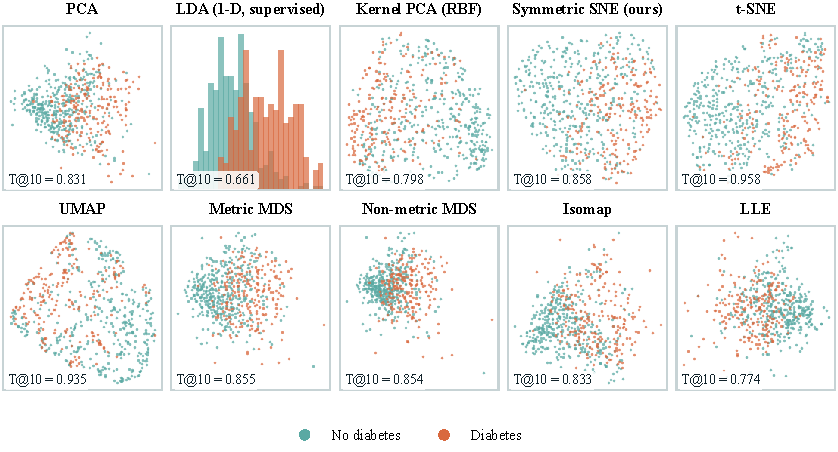
\includegraphics[width=\textwidth]{fig_embeddings}
\caption{Ten reducers on the same 614 development patients, coloured by the known diagnosis (labels are used to fit LDA only). $T@10$ is trustworthiness at $k=10$. The neighbourhood methods (t-SNE, UMAP) give the most structured pictures, but no panel separates the classes better than the raw features do (Fig.~\ref{fig:quality}).}
\label{fig:embeddings}
\vspace{2mm}
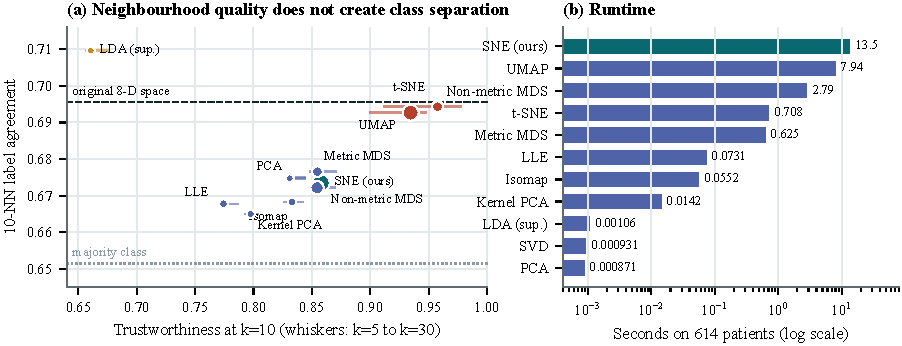
\includegraphics[width=\textwidth]{fig_quality}
\caption{(a) Neighbourhood preservation against class agreement; marker area grows with runtime and whiskers span $k=5$ to $30$. Better neighbourhood preservation does not translate into class separation above the original space (dashed line). (b) Runtime on 614 patients; the from-scratch SNE is the slowest because it is $O(n^2)$ per iteration without approximation.}
\label{fig:quality}
\end{figure*}

\subsection{Baseline classifiers on all eight features}
Table~\ref{tab:baseline} reports the seven classifiers on all eight measurements. Logistic regression is best on both mean five-fold accuracy (0.788) and AUC (0.844). Without the leaked values and duplicated patients, the ranking of the original project reverses: the tree ensembles that led it now trail, with training AUC near 0.98 and validation AUC below 0.84.

\begin{table}[!tb]
\centering
\caption{Seven classifiers on all eight features: mean over five shared outer folds.}
\label{tab:baseline}
\footnotesize
\begin{tabular}{@{}lccc@{}}
\toprule
Classifier & Accuracy & CV AUC & Train AUC \\
\midrule
\textbf{Logistic regression} & \textbf{0.788 $\pm$ 0.020} & \textbf{0.844} & 0.852 \\
Random forest & 0.767 $\pm$ 0.017 & 0.836 & 0.977 \\
SVM (RBF) & 0.764 $\pm$ 0.030 & 0.831 & 0.905 \\
Gaussian naive Bayes & 0.757 $\pm$ 0.026 & 0.831 & 0.838 \\
Gradient boosting & 0.752 $\pm$ 0.008 & 0.820 & 0.982 \\
KNN ($k=7$) & 0.754 $\pm$ 0.043 & 0.810 & 0.893 \\
Decision tree (depth 5) & 0.753 $\pm$ 0.034 & 0.787 & 0.921 \\
\bottomrule
\end{tabular}
\end{table}

\subsection{Embedding quality}
Fig.~\ref{fig:embeddings} shows all ten two-dimensional embeddings and the one-dimensional LDA axis on the same patients, and Table~\ref{tab:emb} and Fig.~\ref{fig:quality} give the measurements. t-SNE preserves neighbourhoods best ($T(10)=0.958$), followed by UMAP (0.935). Our symmetric SNE (0.858) sits about 0.10 below t-SNE; its Gaussian output kernel cannot place moderately distant neighbours far enough apart, so the map collapses into one disc, which is the crowding problem that motivated t-SNE \cite{vandermaaten2008}. Metric and non-metric MDS (0.855) and Isomap (0.833) are close to PCA (0.831). Kernel PCA (0.798) and LLE (0.774) preserve neighbourhoods worst among unsupervised methods.

\begin{figure*}[!t]
\centering
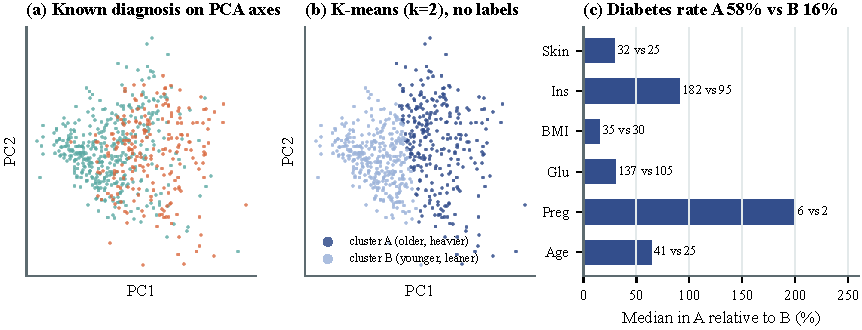
\includegraphics[width=\textwidth]{fig_cluster}
\caption{Clustering without labels. (a) Known diagnosis on PCA axes. (b) K-means clusters on the same axes. (c) Median measurements in cluster A relative to cluster B, with the post-hoc diabetes rates.}
\label{fig:cluster}
\end{figure*}

Class separation tells a different story. Every unsupervised embedding has a 10-NN label agreement between 0.665 and 0.694, at or below the 0.696 of the original eight-dimensional space, against 0.652 for always predicting the majority class. The reducers therefore do not create class structure; the overlap in the t-SNE and UMAP panels is real overlap in the data. Only LDA, which uses the labels, scores higher (0.710), and it does so with the worst trustworthiness (0.661) because one axis cannot preserve neighbourhoods.

\begin{table}[!tb]
\centering
\caption{Embedding quality on 614 patients (two dimensions; LDA one).}
\label{tab:emb}
\footnotesize
\setlength{\tabcolsep}{3.5pt}
\begin{tabular}{@{}lccccr@{}}
\toprule
Method & $T(5)$ & $T(10)$ & $T(30)$ & 10-NN agr. & Sec. \\
\midrule
t-SNE & \textbf{0.977} & \textbf{0.958} & \textbf{0.912} & 0.694 & 0.71 \\
UMAP & 0.947 & 0.935 & 0.900 & 0.693 & 7.94 \\
SNE (ours) & 0.856 & 0.858 & 0.861 & 0.674 & 13.5 \\
Metric MDS & 0.848 & 0.855 & 0.870 & 0.677 & 0.62 \\
Non-metric MDS & 0.851 & 0.854 & 0.870 & 0.672 & 2.79 \\
Isomap & 0.827 & 0.833 & 0.842 & 0.668 & 0.06 \\
PCA & 0.831 & 0.831 & 0.844 & 0.675 & $<$0.01 \\
Truncated SVD & 0.831 & 0.831 & 0.844 & 0.675 & $<$0.01 \\
Kernel PCA & 0.793 & 0.798 & 0.804 & 0.665 & 0.01 \\
LLE & 0.773 & 0.774 & 0.787 & 0.668 & 0.07 \\
LDA (supervised) & 0.657 & 0.661 & 0.675 & \textbf{0.710} & $<$0.01 \\
\midrule
Original 8-D space & \multicolumn{3}{c}{n/a} & 0.696 & \\
\bottomrule
\end{tabular}
\end{table}

\subsection{Clustering}
The silhouette coefficient is highest at $k=2$ but low (0.21), so the data has weak cluster structure. The two clusters separate an older, more often pregnant, heavier, higher-glucose profile (cluster A: median age 41, glucose 137 mg/dL, BMI 34.6) from a younger, leaner one (cluster B: age 25, glucose 105, BMI 30.0) (Fig.~\ref{fig:cluster}). Checked against the diagnosis only afterwards, cluster A is 58\% diabetic and cluster B 16\%. Agreement with the diagnosis is still weak (ARI 0.19, NMI 0.15): 118 of the 279 patients in cluster A are not diabetic and 53 of the 214 diabetic patients fall in cluster B. The clusters describe risk profiles; they do not recover the diagnosis.

\subsection{Prediction: reduction versus selection versus all features}
Fig.~\ref{fig:forest} compares 25 representations with logistic regression as the reference classifier, fixed in advance. Each point is the mean change in outer-CV AUC relative to all eight features, with per-fold differences shown as dots. Fig.~\ref{fig:heat} repeats the comparison for all seven classifiers.

\begin{figure}[!tb]
\centering
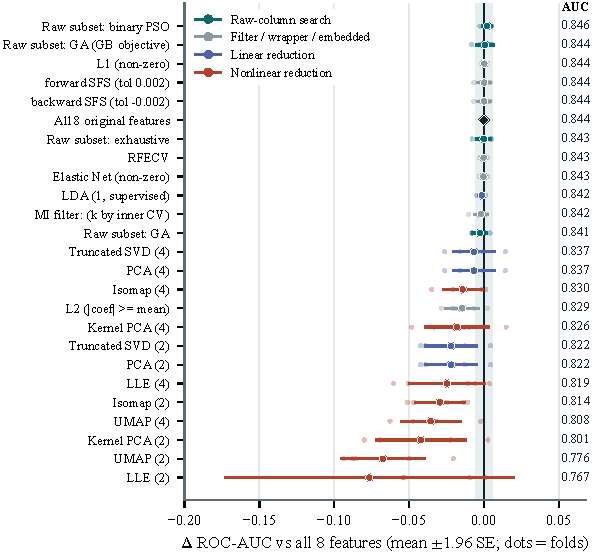
\includegraphics[width=\columnwidth]{fig_forest}
\caption{Change in mean outer-CV AUC relative to all eight features, logistic regression, identical folds. Bars are $\pm1.96$ standard errors of the paired fold differences; the shaded band is $\pm0.005$. Right column: mean CV AUC.}
\label{fig:forest}
\end{figure}

\begin{figure*}[!t]
\centering
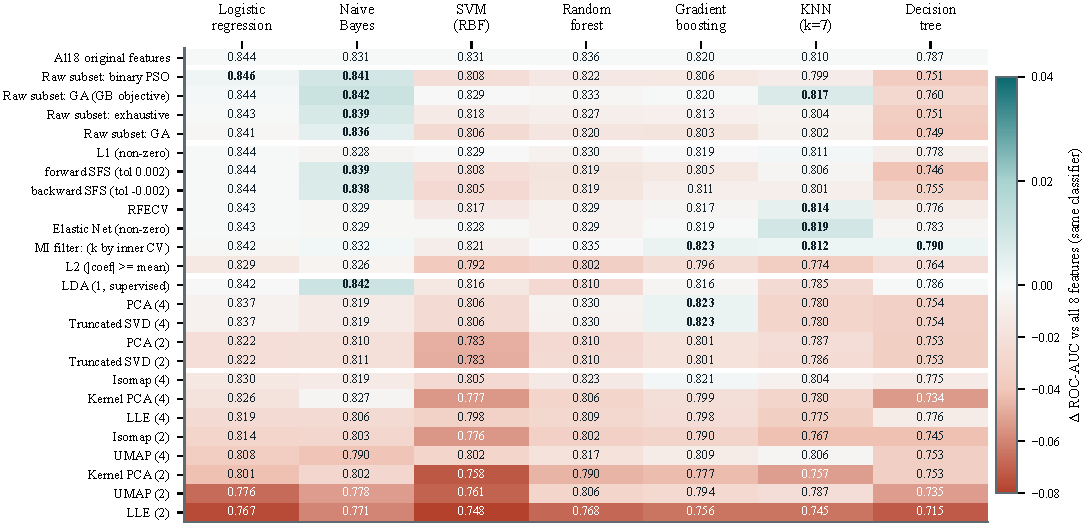
\includegraphics[width=\textwidth]{fig_heat}
\caption{Mean outer-CV AUC for 25 representations (rows) and 7 classifiers (columns); colour is the change relative to all eight features for the same classifier, bold marks gains above 0.002. Rows are grouped as all features, raw-column search, filter/wrapper/embedded, linear and nonlinear reduction. The bottom block is red for every classifier.}
\label{fig:heat}
\end{figure*}

\textit{Nonlinear reduction does not help.} The best nonlinear representation, Isomap with four components, loses 0.014 AUC and 2.3 accuracy points against all eight features. Kernel PCA (4) loses 0.018, LLE (4) 0.025 and UMAP (4) 0.036. At two components the losses grow: UMAP (2) loses 0.068 and LLE (2) 0.077. LLE is also unstable; in some folds its output collapses so that the classifier predicts only the majority class, giving an accuracy of 0.653. No nonlinear representation beats all eight features in more than one of five folds. Across all seven classifiers the best nonlinear change ranges from $-0.026$ (SVM) to $+0.001$ (gradient boosting with Isomap-4), well inside the fold-to-fold noise of about 0.015 to 0.02.

\textit{Linear reduction mostly loses too.} PCA and SVD with four components lose 0.007 AUC and with two components 0.022. The supervised one-dimensional LDA ties with all eight features ($-0.001$), as expected for a model that is itself linear.

\textit{Selection ties at lower cost.} Every filter, wrapper and embedded selector stays within 0.002 AUC of all eight features. The raw-column searches do the same while needing 4.0 to 4.4 measurements instead of 8: the BPSO subset gains 0.002 and wins four of five folds, the GB-objective GA subset gains 0.001, and the exhaustive subset loses 0.0002. Subsets are model-specific, however: the logistic-regression subset costs the decision tree 0.027 AUC (Fig.~\ref{fig:heat}).

\subsection{What the selectors chose}
Fig.~\ref{fig:selection} lists the subsets each selector chose on the full development set and the selection frequencies of GA and BPSO across seeds. Glucose, BMI and pregnancies appear in every subset; the pedigree function in most. With logistic regression, no selector needs insulin or skin fold once a feature must earn 0.002 AUC. This reverses the original project's finding that insulin was selected by every method, which came from the label-derived insulin values. The gradient-boosting objective does keep insulin and age, but a subset without insulin (glucose, BMI, age) comes within 0.0027 of its optimum.

\begin{figure}[!tb]
\centering
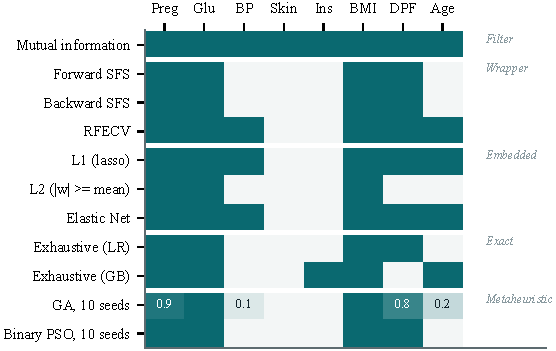
\includegraphics[width=\columnwidth]{fig_selection}
\caption{Features chosen by each selector on the 614 development patients (filled = selected). The last two rows give selection frequencies over ten seeds. Exhaustive rows are the exact optima of \eqref{eq:objective} for each estimator.}
\label{fig:selection}
\end{figure}

\begin{figure*}[!t]
\centering
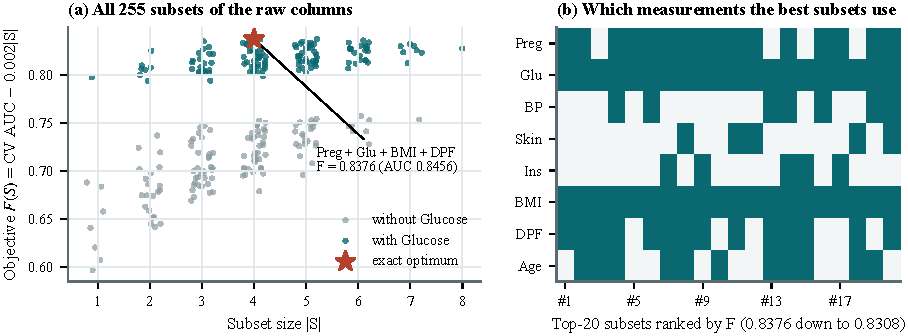
\includegraphics[width=\textwidth]{fig_landscape}
\caption{The full search space. (a) Objective of all 255 subsets by size; subsets with glucose form a separate upper band. (b) Measurements used by the top 20 subsets: glucose and BMI are always present, insulin and skin fold rarely.}
\label{fig:landscape}
\vspace{2mm}
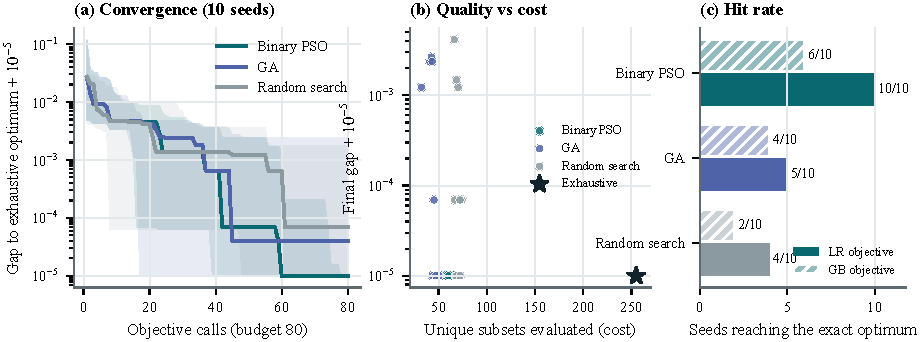
\includegraphics[width=\textwidth]{fig_meta}
\caption{Metaheuristics against the exact optimum (logistic-regression objective unless stated). (a) Gap to $F^\star$ against objective calls, median and 10th to 90th percentile over ten seeds. (b) Final gap against unique subsets evaluated for every run; the star is exhaustive search. (c) Seeds that reached the exact optimum under both objectives.}
\label{fig:meta}
\end{figure*}

\subsection{GA versus binary PSO against the exact optimum}
Exhaustive search over the 255 subsets took 13.5 s with logistic regression. Its optimum is \{pregnancies, glucose, BMI, DPF\} with $F^\star=0.8376$ (CV AUC 0.8456). Fig.~\ref{fig:landscape} shows why searching this space is easy and choosing within it is hard: every good subset contains glucose, and the top 20 subsets span only 0.007 in $F$.

Table~\ref{tab:meta} and Fig.~\ref{fig:meta} give the comparison under equal budget. With the logistic-regression objective BPSO found the exact optimum in all ten seeds, evaluating on average 63 unique subsets, 25\% of the exhaustive cost, and reaching the optimum after about 48. The GA converged faster, settling on its final answer after about 22 unique subsets, but reached the optimum in only five of ten seeds; its misses were neighbouring subsets within 0.0026. Random search with the same budget reached the optimum in four of ten. Under the gradient-boosting objective, whose landscape is noisier, BPSO hit the optimum in six of ten seeds, the GA in four and random search in two, and the exhaustive search costs about 200 s on one core.

\begin{table}[!tb]
\centering
\caption{Search quality and cost over ten seeds (budget: 80 objective calls). ``Unique'' is the number of distinct subsets evaluated, the real cost; ``To best'' is unique subsets until the final best was first found.}
\label{tab:meta}
\footnotesize
\setlength{\tabcolsep}{3pt}
\begin{tabular}{@{}llccccc@{}}
\toprule
Obj. & Algorithm & Hit & Mean gap & Unique & To best & Distinct \\
\midrule
\multirow{4}{*}{LR} & \textbf{Binary PSO} & \textbf{10/10} & \textbf{0.0000} & 63.0 & 48.3 & 1 \\
 & GA & 5/10 & 0.0009 & 44.3 & 21.6 & 5 \\
 & Random search & 4/10 & 0.0007 & 69.8 & 34.7 & 5 \\
 & Exhaustive & exact & 0 & 255 & n/a & 1 \\
\midrule
\multirow{4}{*}{GB} & \textbf{Binary PSO} & \textbf{6/10} & \textbf{0.0010} & 62.7 & 43.4 & 4 \\
 & GA & 4/10 & 0.0022 & 45.4 & 29.7 & 5 \\
 & Random search & 2/10 & 0.0024 & 69.8 & 32.0 & 4 \\
 & Exhaustive & exact & 0 & 255 & n/a & 1 \\
\bottomrule
\end{tabular}
\end{table}

Inside the nested outer folds, with one seed and the same budget, the GA reached the inner-CV optimum in three of five folds (about 38 unique subsets) and BPSO in two of five (about 60). Every miss was within 0.003 and differed from the optimum by one feature, usually age or DPF. The outer AUC did not suffer: the BPSO pipeline (0.8458) even scored above the always-exact exhaustive pipeline (0.8435). Optimizing the inner objective more exactly does not buy held-out performance at this scale; differences of a few thousandths are noise.

\begin{figure*}[!t]
\centering
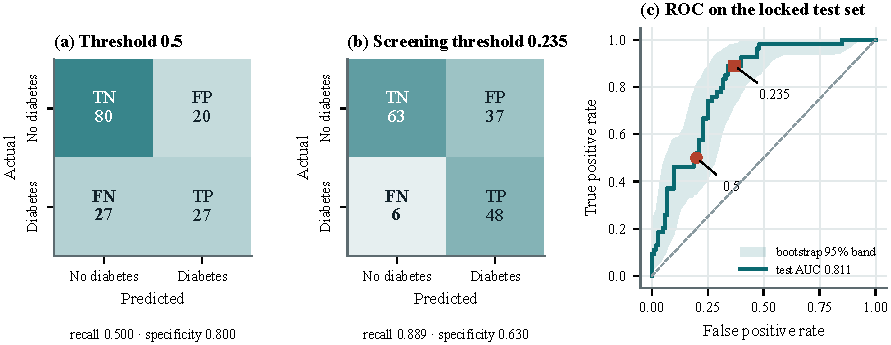
\includegraphics[width=\textwidth]{fig_final}
\caption{The locked test set (154 patients). (a, b) Confusion matrices at the default and the pre-set screening threshold. (c) ROC curve with a bootstrap 95\% band; markers show the two operating points.}
\label{fig:final}
\end{figure*}

\subsection{Leaderboard and finalist}
Table~\ref{tab:leader} lists the top of the 181-pipeline leaderboard. The pre-set rule selects logistic regression on the BPSO-selected raw columns. Refitted on all 614 development patients, BPSO chose pregnancies, glucose, BMI and DPF, the exhaustive optimum. Eighteen pipelines fall within one standard error (0.0068) of the top, including logistic regression on all eight features, so the finalist does not predict measurably better than the all-feature model; what it offers is the same accuracy from half the measurements. Nested tuning narrows the overfitting of the flexible models without beating logistic regression: tuned gradient boosting reaches 0.834 AUC and the tuned random forest 0.837. The honest replica of the original pipeline scores 0.829 AUC and 75.9\% accuracy, against the 0.942 and 87.8\% it reported.

\begin{table}[!tb]
\centering
\caption{Top of the leaderboard (181 pipelines, identical outer folds) and the original pipeline re-estimated.}
\label{tab:leader}
\footnotesize
\setlength{\tabcolsep}{3pt}
\begin{tabular}{@{}llccc@{}}
\toprule
Representation & Classifier & Raw & CV AUC & CV acc. \\
\midrule
\textbf{BPSO raw subset} & \textbf{LR} & \textbf{4.2} & \textbf{0.846} & \textbf{0.792} \\
All 8 (tuned) & LR, tuned $C$ & 8 & 0.844 & 0.787 \\
GA (GB obj.) raw subset & LR & 4.0 & 0.844 & 0.790 \\
All 8 (tuned) & SVM, tuned & 8 & 0.844 & 0.787 \\
L1 selection & LR & 8 & 0.844 & 0.787 \\
Forward SFS & LR & 8 & 0.844 & 0.793 \\
Backward SFS & LR & 8 & 0.844 & 0.796 \\
All 8 features & LR & 8 & 0.844 & 0.788 \\
Exhaustive raw subset & LR & 4.4 & 0.843 & 0.790 \\
\midrule
Original pipeline, nested & GB, tuned & 5.0 & 0.829 & 0.759 \\
\bottomrule
\multicolumn{5}{@{}l}{\scriptsize ``Raw'': mean number of raw measurements the pipeline needs across folds.}
\end{tabular}
\end{table}

\subsection{Final evaluation on the locked test set}
The screening threshold chosen from out-of-fold development predictions is 0.235 (out-of-fold recall 0.851, specificity 0.620). The test set was then opened once. Table~\ref{tab:final} and Fig.~\ref{fig:final} report the results.

\begin{table}[!tb]
\centering
\caption{Finalist (LR on pregnancies, glucose, BMI, DPF). Test intervals are 2,000-sample bootstrap 95\% CIs.}
\label{tab:final}
\footnotesize
\setlength{\tabcolsep}{3pt}
\begin{tabular}{@{}lccc@{}}
\toprule
 & Dev OOF, 0.5 & Test, 0.5 & Test, 0.235 \\
\midrule
TN / FP / FN / TP & 360/40/88/126 & 80/20/27/27 & 63/37/6/48 \\
Accuracy & 0.792 & 0.695 {\scriptsize(0.62--0.77)} & 0.721 {\scriptsize(0.65--0.79)} \\
Error rate & 0.208 & 0.305 & 0.279 \\
Precision & 0.759 & 0.574 & 0.565 \\
Recall & 0.589 & 0.500 {\scriptsize(0.37--0.63)} & \textbf{0.889} {\scriptsize(0.80--0.97)} \\
Specificity & 0.900 & 0.800 & 0.630 {\scriptsize(0.53--0.72)} \\
F1 & 0.663 & 0.535 & 0.691 \\
ROC-AUC & 0.847 & \multicolumn{2}{c}{0.811 {\scriptsize(0.736--0.871)}} \\
\bottomrule
\end{tabular}
\end{table}

\textit{Reading the confusion matrices.} At 0.5 the model misses 27 of 54 diabetic patients. Their measurements look healthy: median glucose 123 mg/dL against 164 for the diabetic patients it detects, BMI 32.0 against 36.6 and age 32 against 38. The screening threshold catches 21 of these 27 at the cost of 17 additional false alarms. The six diabetic patients still missed have glucose between 78 and 129 mg/dL, and four of them lack insulin or skin-fold values, so with these measurements they cannot be told apart from healthy patients. The 20 false positives at 0.5 look diabetic (median glucose 153.5 mg/dL, BMI 37.5). In screening each costs a confirmatory glucose test, which is much cheaper than a missed diagnosis.

\subsection{Overfitting, underfitting and the test gap}
Fig.~\ref{fig:fit} contrasts training-fold and validation AUC. The finalist is not overfitted: training AUC 0.850, out-of-fold 0.847. Its learning curve on the outer folds levels off at a validation AUC of about 0.845 from roughly 250 training patients while training AUC falls to meet it. This is a high-bias regime in which the limit is the information in the measurements, so more flexible models only overfit: gradient boosting reaches a training AUC of 0.982 for a validation AUC of 0.820, the random forest 0.977 for 0.836, and tuned KNN with distance weights memorizes the training folds completely (1.000 for 0.830).

\begin{figure}[!tb]
\centering
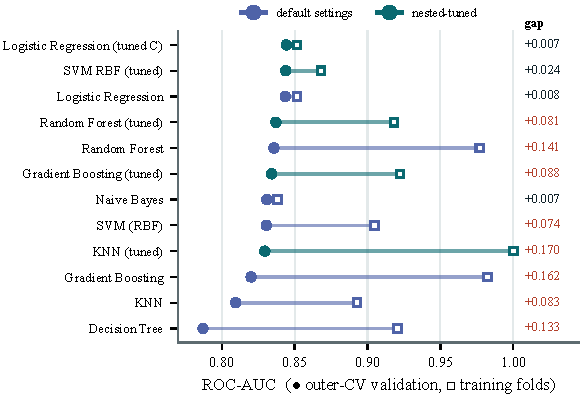
\includegraphics[width=\columnwidth]{fig_fit}
\caption{Training-fold versus validation AUC on all eight features. Right column: the gap. Linear models and naive Bayes fit without overfitting; tree ensembles and KNN overfit by 0.07 to 0.17 AUC without gaining validation AUC.}
\label{fig:fit}
\end{figure}

The test AUC (0.811) and accuracy (0.695) are below their CV estimates. After the finalist was locked, four other pipelines were refitted and scored on the same test patients; this diagnostic could not change the choice. All five lose between 0.016 and 0.038 AUC (Fig.~\ref{fig:compare}a), and the finalist's loss of 0.035 is typical, so the gap comes from this particular 154-patient split and not from overfitting of the finalist. With 154 patients one accuracy point is 1.5 patients, and the bootstrap interval for test AUC (0.736 to 0.871) contains the CV estimate.

\begin{figure*}[!t]
\centering
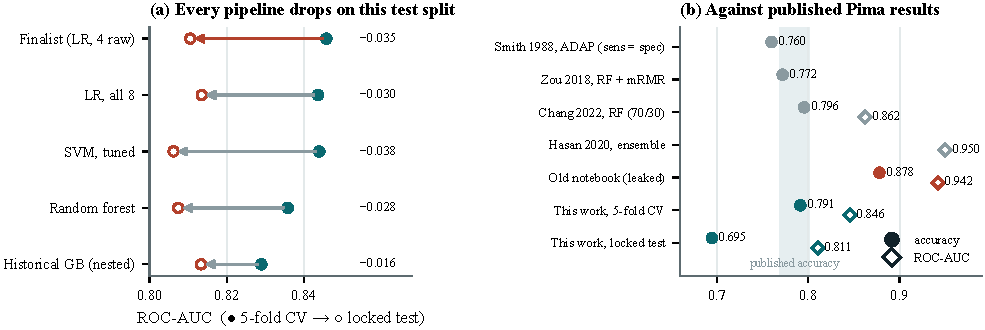
\includegraphics[width=\textwidth]{fig_compare}
\caption{(a) Cross-validated (filled) and locked-test (open) AUC for the finalist and four reference pipelines refitted after the finalist was locked: every pipeline drops on this split. (b) Reported accuracy (circles) and AUC (diamonds) of verified Pima studies, the leaked original pipeline and this work; the shaded band is the 77--80\% accuracy range of the verified single-classifier studies.}
\label{fig:compare}
\end{figure*}

\subsection{Comparison with published results}
Fig.~\ref{fig:compare}b places the results next to the verified studies of Table~\ref{tab:related}. The corrected CV accuracy of 79.2\% falls inside the 77--80\% range of the single-classifier studies \cite{zou2018,chang2022}. The CV AUC of 0.846 is below Chang \textit{et al.}'s 0.862 from a single split and Hasan \textit{et al.}'s 0.950 from an ensemble with outlier rejection, both of which use protocols we could not reproduce exactly. The leaked original result sits eight to ten accuracy points above the verified range, which is consistent with the size of the leak found in Section~\ref{sec:data}.

%======================================================================
\section{Discussion}
%======================================================================

\subsection{How the leak produced plausible numbers}
None of the original faults was exotic. Downloading a ``cleaned'' copy, merging two versions to get more rows and reading the best threshold off a results table are common steps in student and applied work. Each one inflated the score in a way that looked like a modelling success: the tree ensembles appeared to win because they can memorize near-duplicate patients and the class-specific insulin values, and insulin appeared to be the second most important feature because its filled values were the label. The audit took less effort than the modelling and changed every conclusion of the original study. A short checklist would have caught all three faults: confirm that row counts match the documented cohort, compare file versions column by column before merging, and check whether any imputed value is constant within a class.

\subsection{Why nonlinear reduction does not help here}
The Pima features are few, mostly unimodal and only weakly correlated, and the class signal is largely monotone in glucose and BMI. A linear model already captures that signal, which is why LDA's single axis matches all eight features. Nonlinear reducers optimize for something else: t-SNE and UMAP preserve local neighbourhoods, and Isomap and LLE assume a low-dimensional manifold. On this data those goals discard part of the monotone signal, and the losses grow as the number of retained dimensions falls. The embeddings are still useful for showing that the classes overlap and that the clusters correspond to age and body-size profiles; Table~\ref{tab:emb} shows that their pictures should not be read as evidence of separability.

\subsection{When metaheuristics are worth it}
BPSO's ten-of-ten hit rate and the GA's five-of-ten are consistent with the shapes of their searches. BPSO keeps sampling around personal and global bests through all iterations, using more unique evaluations and exploring longer; the GA's tournament selection and elitism concentrate the population quickly, so it spends less but sometimes stops on a neighbour of the optimum. Both beat random search at equal budget. With eight features, though, exhaustive search is exact and costs 13.5 s, so it is the right tool for this dataset, and the metaheuristics are best read as validated against it. The nested results add a practical point: exact optimization of a noisy cross-validated objective did not improve held-out AUC, because the top subsets are within noise of each other. A metaheuristic becomes necessary once the number of candidate features makes exhaustive search impossible; the evidence here supports BPSO over this GA configuration for that case.

\subsection{Clinical reading}
The finalist uses four measurements that are routine and rarely missing: the number of pregnancies, a 2-hour glucose value, BMI and a family-history score. It drops insulin and skin fold, which are missing for 49\% and 30\% of patients. At the pre-set threshold it detects 89\% of diabetic patients at a specificity of 63\%, an acceptable trade for a first-stage screen followed by a confirmatory test. The remaining misses have normal glucose, so no model built on these measurements is likely to catch them.

\subsection{Limitations}
The study uses one cohort from one population, without external validation. The test set is small, so test metrics have wide intervals. The original cleaned file was unavailable, so its construction was established by exact reproduction of the original outputs rather than by comparing bytes. Of the related studies, Hasan \textit{et al.} could be verified only from its abstract. Nested searches used one seed per fold; more seeds would tighten the nested hit-rate estimates.

%======================================================================
\section{Conclusion}
%======================================================================

A leakage audit of a Pima diabetes pipeline that reported 87.8\% accuracy found two copies of the same patients, a label-derived insulin fill and test-set model selection; under a leakage-free protocol the same pipeline scores 75.9\%. On that protocol, nonlinear dimensionality reduction did not improve prediction for any of seven classifiers, filter, wrapper and embedded selection tied with all eight features, and binary PSO found the exact best subset in every seed at a quarter of the exhaustive cost while the GA did so in half. Logistic regression on four routine measurements gives a cross-validated AUC of 0.846 and accuracy of 79.2\%, a locked-test AUC of 0.811, and 89\% sensitivity at a screening threshold chosen without the test set. The main lesson for small clinical benchmarks is to verify the data and lock the evaluation before comparing methods: here that step changed every conclusion.

\section*{Data and Code Availability}
The verified data, the executed notebook, the figure script and all result tables are available at \url{https://github.com/ziadmohamdd/PimaLens}.

\section*{Acknowledgment}
This work was carried out for the course AID427 New Trends in Data Science at the Egypt-Japan University of Science and Technology.

% Output every pending figure and table so none lands inside the reference list.
\clearpage

\begin{thebibliography}{99}

\bibitem{smith1988} J.~W. Smith, J.~E. Everhart, W.~C. Dickson, W.~C. Knowler, and R.~S. Johannes, ``Using the ADAP learning algorithm to forecast the onset of diabetes mellitus,'' in \textit{Proc. Annu. Symp. Comput. Appl. Med. Care}, 1988, pp.~261--265.

\bibitem{uci_pima} V.~Sigillito, ``Pima Indians Diabetes Database,'' UCI Machine Learning Repository, 1990. Available as OpenML dataset 37, \url{https://www.openml.org/d/37}.

\bibitem{zou2018} Q.~Zou, K.~Qu, Y.~Luo, D.~Yin, Y.~Ju, and H.~Tang, ``Predicting diabetes mellitus with machine learning techniques,'' \textit{Front. Genet.}, vol.~9, p.~515, 2018.

\bibitem{chang2022} V.~Chang, J.~Bailey, Q.~A. Xu, and Z.~Sun, ``Pima Indians diabetes mellitus classification based on machine learning (ML) algorithms,'' \textit{Neural Comput. Appl.}, 2022, doi: 10.1007/s00521-022-07049-z.

\bibitem{hasan2020} M.~K. Hasan, M.~A. Alam, D.~Das, E.~Hossain, and M.~Hasan, ``Diabetes prediction using ensembling of different machine learning classifiers,'' \textit{IEEE Access}, vol.~8, pp.~76516--76531, 2020.

\bibitem{kapoor2023} S.~Kapoor and A.~Narayanan, ``Leakage and the reproducibility crisis in machine-learning-based science,'' \textit{Patterns}, vol.~4, no.~9, p.~100804, 2023.

\bibitem{cawley2010} G.~C. Cawley and N.~L.~C. Talbot, ``On over-fitting in model selection and subsequent selection bias in performance evaluation,'' \textit{J. Mach. Learn. Res.}, vol.~11, pp.~2079--2107, 2010.

\bibitem{ambroise2002} C.~Ambroise and G.~J. McLachlan, ``Selection bias in gene extraction on the basis of microarray gene-expression data,'' \textit{Proc. Natl. Acad. Sci. USA}, vol.~99, no.~10, pp.~6562--6566, 2002.

\bibitem{varma2006} S.~Varma and R.~Simon, ``Bias in error estimation when using cross-validation for model selection,'' \textit{BMC Bioinformatics}, vol.~7, p.~91, 2006.

\bibitem{scholkopf1998} B.~Sch\"{o}lkopf, A.~Smola, and K.-R. M\"{u}ller, ``Nonlinear component analysis as a kernel eigenvalue problem,'' \textit{Neural Comput.}, vol.~10, no.~5, pp.~1299--1319, 1998.

\bibitem{kruskal1964} J.~B. Kruskal, ``Nonmetric multidimensional scaling: A numerical method,'' \textit{Psychometrika}, vol.~29, no.~2, pp.~115--129, 1964.

\bibitem{tenenbaum2000} J.~B. Tenenbaum, V.~de~Silva, and J.~C. Langford, ``A global geometric framework for nonlinear dimensionality reduction,'' \textit{Science}, vol.~290, pp.~2319--2323, 2000.

\bibitem{roweis2000} S.~T. Roweis and L.~K. Saul, ``Nonlinear dimensionality reduction by locally linear embedding,'' \textit{Science}, vol.~290, pp.~2323--2326, 2000.

\bibitem{hinton2002} G.~E. Hinton and S.~T. Roweis, ``Stochastic neighbor embedding,'' in \textit{Adv. Neural Inf. Process. Syst.}, vol.~15, 2002.

\bibitem{vandermaaten2008} L.~van der Maaten and G.~Hinton, ``Visualizing data using t-SNE,'' \textit{J. Mach. Learn. Res.}, vol.~9, pp.~2579--2605, 2008.

\bibitem{mcinnes2018} L.~McInnes, J.~Healy, and J.~Melville, ``UMAP: Uniform manifold approximation and projection for dimension reduction,'' arXiv:1802.03426, 2018.

\bibitem{venna2001} J.~Venna and S.~Kaski, ``Neighborhood preservation in nonlinear projection methods: An experimental study,'' in \textit{Proc. Int. Conf. Artif. Neural Netw. (ICANN)}, 2001, pp.~485--491.

\bibitem{holland1975} J.~H. Holland, \textit{Adaptation in Natural and Artificial Systems}. Ann Arbor, MI, USA: Univ. Michigan Press, 1975.

\bibitem{kennedy1997} J.~Kennedy and R.~C. Eberhart, ``A discrete binary version of the particle swarm algorithm,'' in \textit{Proc. IEEE Int. Conf. Syst., Man, Cybern.}, 1997, pp.~4104--4108.

\bibitem{clerc2002} M.~Clerc and J.~Kennedy, ``The particle swarm: Explosion, stability, and convergence in a multidimensional complex space,'' \textit{IEEE Trans. Evol. Comput.}, vol.~6, no.~1, pp.~58--73, 2002.

\bibitem{xue2016} B.~Xue, M.~Zhang, W.~N. Browne, and X.~Yao, ``A survey on evolutionary computation approaches to feature selection,'' \textit{IEEE Trans. Evol. Comput.}, vol.~20, no.~4, pp.~606--626, 2016.

\bibitem{troyanskaya2001} O.~Troyanskaya \textit{et al.}, ``Missing value estimation methods for DNA microarrays,'' \textit{Bioinformatics}, vol.~17, no.~6, pp.~520--525, 2001.

\bibitem{kraskov2004} A.~Kraskov, H.~St\"{o}gbauer, and P.~Grassberger, ``Estimating mutual information,'' \textit{Phys. Rev. E}, vol.~69, p.~066138, 2004.

\bibitem{guyon2002} I.~Guyon, J.~Weston, S.~Barnhill, and V.~Vapnik, ``Gene selection for cancer classification using support vector machines,'' \textit{Mach. Learn.}, vol.~46, pp.~389--422, 2002.

\bibitem{tibshirani1996} R.~Tibshirani, ``Regression shrinkage and selection via the lasso,'' \textit{J. R. Stat. Soc. B}, vol.~58, no.~1, pp.~267--288, 1996.

\bibitem{zou2005} H.~Zou and T.~Hastie, ``Regularization and variable selection via the elastic net,'' \textit{J. R. Stat. Soc. B}, vol.~67, no.~2, pp.~301--320, 2005.

\bibitem{cortes1995} C.~Cortes and V.~Vapnik, ``Support-vector networks,'' \textit{Mach. Learn.}, vol.~20, pp.~273--297, 1995.

\bibitem{breiman2001} L.~Breiman, ``Random forests,'' \textit{Mach. Learn.}, vol.~45, pp.~5--32, 2001.

\bibitem{friedman2001} J.~H. Friedman, ``Greedy function approximation: A gradient boosting machine,'' \textit{Ann. Statist.}, vol.~29, no.~5, pp.~1189--1232, 2001.

\end{thebibliography}

\end{document}
